\documentclass[12pt,a4paper]{article}
\usepackage[utf8]{inputenc}
\usepackage[german]{babel}
\usepackage[T1]{fontenc}
\usepackage{amsmath}
\usepackage{amsfonts}
\usepackage{amssymb}
\usepackage{graphicx}
\usepackage[left=2.5cm,right=2.5cm,top=2cm,bottom=2cm]{geometry}
\author{Gruppe C14 \\ Julián Häck, Martin Koytek, Lars Wenning, Erik Zimmermann}
\usepackage{float}
\begin{document}
\section{Schwebung}
Wenn man die D-Saite verstimmt, ist beim Anschlagen der D-Saite leer und der A-Saite im 5. Bund eine Schwebung hörbar.
\begin{figure}[H]
\centering
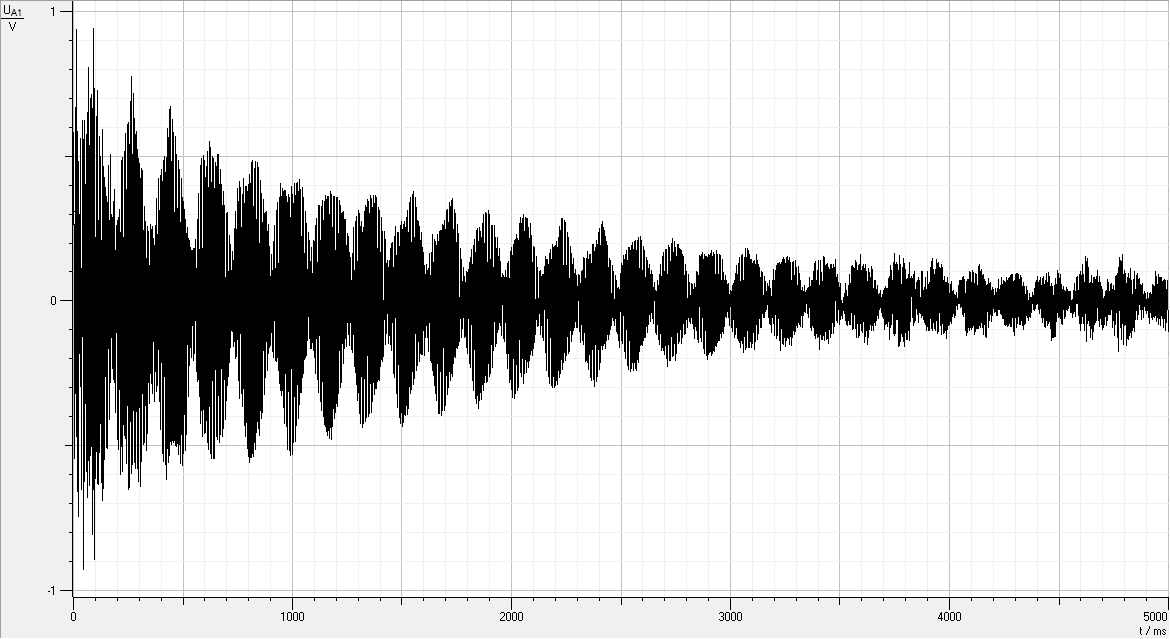
\includegraphics[scale=0.5]{schwebung/Schwebung_Roh.png}
\caption{Gesamte Schwebung}
\end{figure}

Die Frequenz dieser Schwebung wird im Folgenden sowohl durch eine Fast-Fourier-Transformation als auch durch Ablesen der Plots bestimmt werden.

\subsection{Bestimmung der Schwebungsfrequenz durch FFT}
Transformiert man die Schwingung in den Frequenzraum, werden 2 Peaks deutlich. Die kleinere so bestimmte Frequenz bezeichnen wir hier mit $f_-$ die größere mit $f_+$.
\begin{figure}[H]
\centering
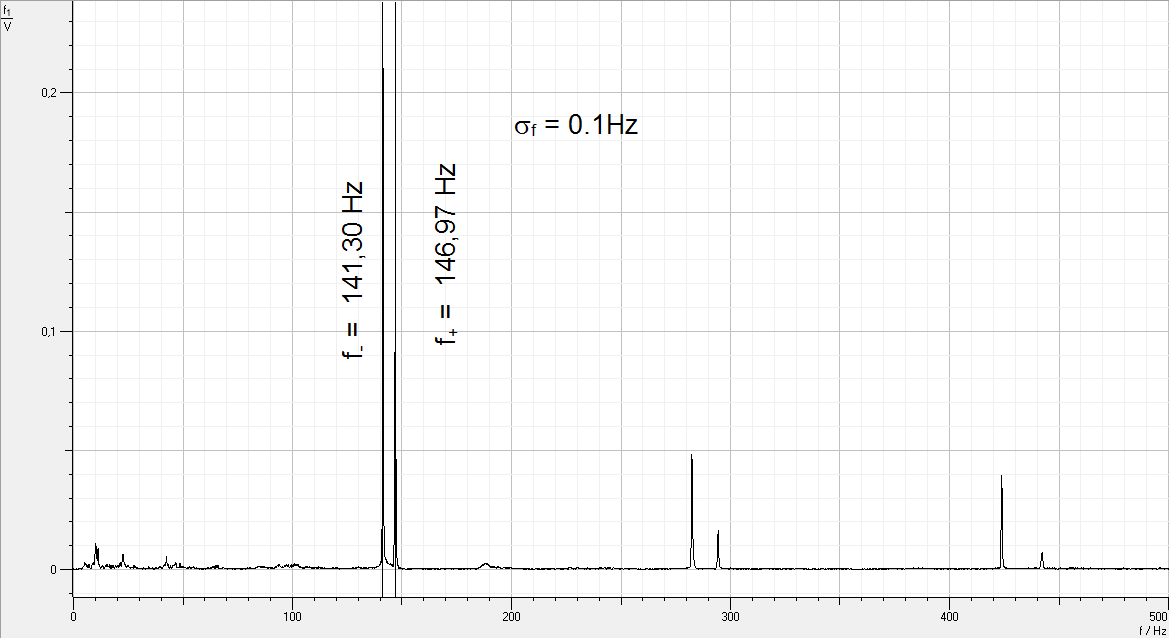
\includegraphics[scale=0.5]{schwebung/Schwebung_FFT.png}
\caption{Bestimmung der Schwebungsfrequenz durch FFT}
\end{figure}

\begin{equation}
f_-=141.3 Hz, \hspace{1cm} f_+=147.0 Hz
\end{equation}

Den Fehler für die FFT haben wir als Ablesefehler zu $ \sigma_f=0.1Hz$ bestimmt.

Mittels
\begin{align}
f_{res}=\frac{f_+ + f_-}{2} \\
f_{sch}=\frac{f_+ - f_-}{2} \\
\sigma_{f_{res}}=\frac{1}{\sqrt{2}}\sigma_f=\sigma_{f_{sch}}
\end{align}
können daraus die resultierende(res) Frequenz und die  Schwebungsfrequenz(sch) und deren Fehler mittels Fehlerfortpflanzung bestimmt werden:

\begin{align}
f_{res}=144.15 \pm 0.07 Hz\\
f_{sch}=2.85 \pm 0.07 Hz
\end{align}

\subsection{Bestimmung der Schwebungsfrequenz durch Ablesen}

Die resultierende Frequenz und die Schwebungsfrequenz können alternativ auch durch Ablesen der Nullstellen bestimmt werden. Dabei gilt:
\begin{equation}
f=\frac{n}{t_e-t_a}.
\end{equation}
\begin{equation}
\sigma_f=\frac{\sqrt{2}n\sigma_t}{(t_e-t_a)^2}
\end{equation}
Mit der Anzahl der Perioden $n$, $t_a$ der Zeit eines möglichst frühen Nulldurchlaufs und $t_e$ der Zeit eines möglichst späten Nulldurchlaufs. 
\begin{figure}[H]
\centering
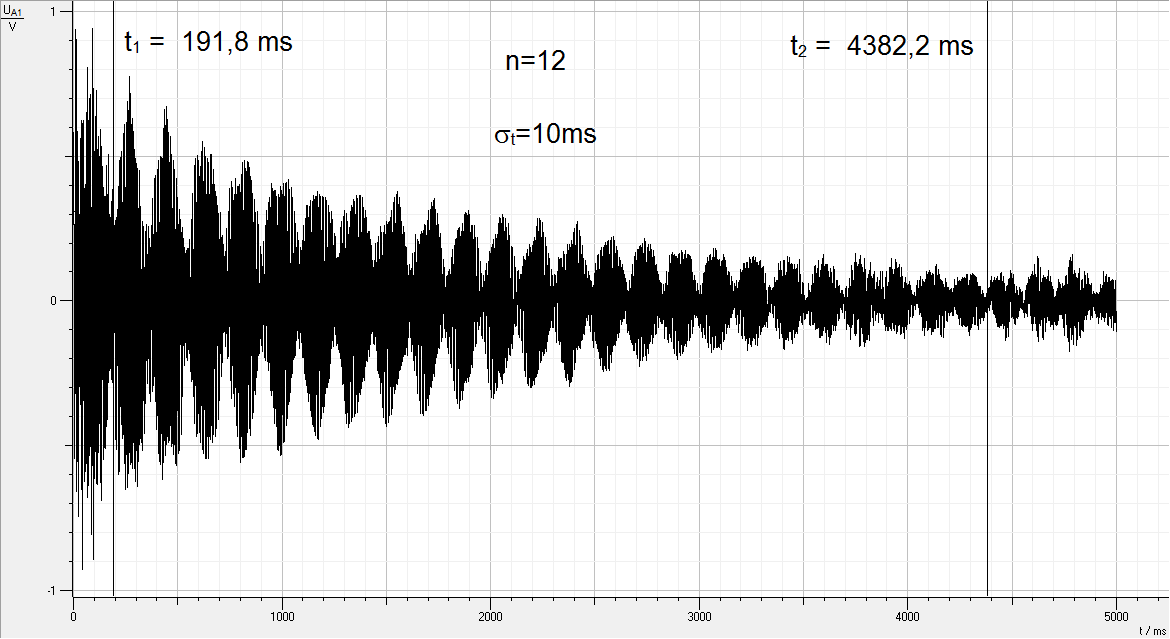
\includegraphics[scale=0.5]{schwebung/Schwebung_ganz_bearb.png}
\caption{Frequenzmessung der Schwebungsfrequenz}
\end{figure}
Der Fehler von $\sigma_t=10ms$ auf die Zeit wurde hier aufgrund der Unschärfe des Plots abgeschätzt. Daraus folgt direkt
\begin{equation}
f_{sch}=2.86 \pm 0.01 Hz.
\end{equation}

\begin{figure}[H]
\centering
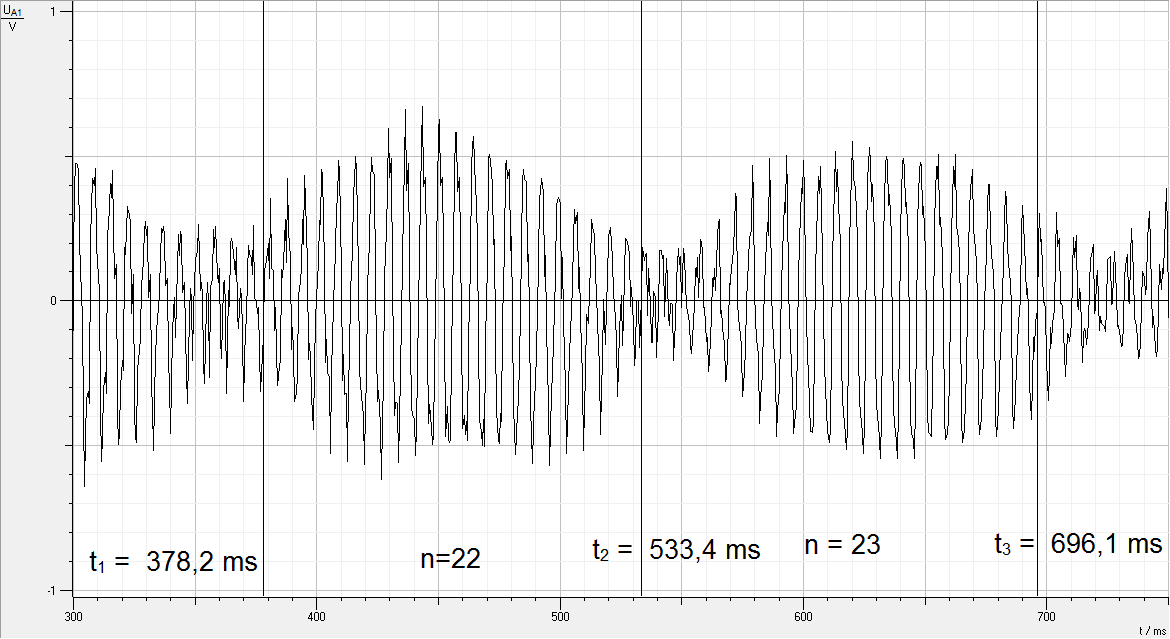
\includegraphics[scale=0.5]{schwebung/Schwebung_zaehlen_2.png}
\caption{Frequenzmessung der Resultierenden}
\end{figure}
Aufgrund der Auflösung des Plots wurde der Fehler auf die  Zeit auf $\sigma_t=1ms$ abgeschätzt.
\begin{equation}
f_{res}=141.55 \pm 0.63Hz.
\end{equation}

\subsection{Fazit}

\begin{table}[H]\centering
\caption{Ergebnis}
\begin{tabular}{c|cc} 
 & FFT & Ablesen \\ 
\hline
$f_{res}$ & $144.15 \pm 0.07 Hz$
 & $141.55 \pm 0.63 Hz$ \\ 
$f_{sch}$ & $2.85 \pm 0.07 Hz$ & $2.86 \pm 0.01 Hz$ \\ 
\end{tabular}
\end{table}
 
Die Frequenzen der resultierenden weichen mit $3.71 \sigma$ voneinander ab wenn man beide Fehler kombiniert. Dass diese Werte voneinander Abweichen lässt sich dadurch erklären, dass die Nulldurchgänge aus einem sehr undeutlichen Plot abzulesen waren. Bei der Frequenzmessung der Resultierenden beispielsweise liegen die vermeintlichen Nullpunkte fast auf demselben Zeitpunkt wie die Maxima. \newline Die Frequenzen der Schwebung sind innerhalb von einem $\sigma$ miteinander verträglich. 

\end{document}